\chapter{QuACKs}
\label{sec:quack}

As previously illustrated, a Sidekick needs to be able to refer to and efficiently
acknowledge a set of opaque packets seen by a network intermediary.
But this problem is technically challenging for middleboxes without access to
cleartext sequence numbers or the ossification of other fields.

We start by mathematically defining the quACK problem.
We discuss how to select an \emph{identifier} to refer to a packet,
and analyze strawman solutions to the quACK problem
that use too much space or computation.
Finally, we present an efficient construction of a quACK based on the insight
that we can model the problem as a system of power sum polynomial equations
when we have a bound on the maximum number of missing elements, a threshold $t$.
This solution is most similar to the deterministic solution to the
\emph{straggler identification} problem~\cite{eppstein2011straggler}, and also builds on
related theoretical work in set reconciliation~\cite{minsky2003set}, and coding
theory and graph theory~\cite{karpovsky2003data}.

Concretely realized, the quACK expresses the equivalent of TCP's
cumulative + selective ACK over opaque (randomly identified) packets
in 48 bytes, tolerating up to 10 missing packets before the last
``selective ACK.'' On a recent x86-64 CPU, it takes 33 ns/packet for a Sidekick PEP
to encode a quACK, and 3~$\mu$s for an end host to decode it. These
overheads compared well with several alternatives (\Cref{sec:quack:microbenchmarks}).

\section{The QuACK Problem}
\label{sec:quack:problem}

We first describe the quACK problem. A data sender transmits a multiset\footnote
{A ``multiset'' means the same element can be transmitted more than once.} of
elements $S$ (these correspond to packets). At any given time, a receiver
(such as a proxy server) has received a subset $R \subseteq S$ of the sent
elements. We would like the receiver to communicate a small amount of
information to the sender, who then efficiently decodes the missing
elements---the set difference $S \setminus R$---knowing $S$. We call this small
amount of information the ``quACK'', and the problem is:
\textbf{what is in a quACK and how do we decode it?}

\paragraph{Packet identifiers.}

In a networking context, how exactly do we refer to the elements
in the quACK problem that have been sent or received?
Traditional TCP middleboxes have been able to interpose their
own concise, cumulative acknowledgments using cleartext sequence numbers, but
this is not possible with modern, secure transport protocols. Even if a
connection did expose an unencrypted numerical field, we would not want to
refer to that field at risk of ossifying that protocol.

Instead, we need a function that deterministically maps
a packet to a random $b$-byte \emph{identifier}. The most trivial solution
that applies to all base protocols is
to hash the entire payload. Another option if the payload is already
pseudorandom (e.g., QUIC) is to take the first $b$ bytes from a fixed
offset of that payload. Although the latter option would rely on those bytes
to remain pseudorandom, it is computationally more efficient because it
does not require reading the entire payload.

\paragraph{Collisions.}
The main considerations when selecting the number of bytes, $b$, in an
identifier is the tolerance for collisions compared with the extra data
needed to refer to these packets on the link. The larger $b$ is, the lower
the collision probability but the greater the link overhead.

Define the collision probability to be the probability that a randomly-chosen
$b$-byte identifier in a list of $n$ packets maps to more than one packet in
that list.
If we assume that identifiers are uniformly distributed,
this probability is equal to $1-(1 - 1/256^{b})^{n-1}$.
When $n=25$, using $4$ bytes results in an almost negligible chance of
collision while using $2$ bytes results in a 0.04\% chance
(\Cref{tab:collision-prob}).
\begin{table}[ht]
  \centering
  \begin{tabular}{|l|l|l|l|l|}
    \hline
    \textbf{Identifier Bytes} & 1 & 2 & 4 & 8 \\
    \hline
    \textbf{Collision Prob.}
    & 0.090 & 0.0004 & $5.6\text{e-09}$ & ${\approx}0$ \\
    \hline
  \end{tabular}
  \caption{Collision probabilities for $n=25$.
  }
  \label{tab:collision-prob}
\end{table}


When handling collisions, a sender who is decoding a quACK has a list of $n$
packets it is trying to classify as received or missing
(\Cref{sec:quack:microbenchmarks}). Note that collisions are also known to the
sender beforehand. If there is a collision between a packet that is received
and a packet that is missing, the fate of that identifier is considered
indeterminate. Either the protocol can still function with approximate
statistics (e.g., congestion control) or it can fall back to an end-to-end
mechanism (e.g., retransmission).

\section{Strawman solutions}
\label{sec:quack:strawmen}

\begin{table*}[h]
  \centering
  % \renewcommand{\arraystretch}{0.000023}
  \small
  \begin{tabular}{llllll}
    \toprule
    & \bf & \bf & \bf Num Additional & \bf Packet Payload & \bf Cumu-\\
    & \bf Per-Packet Encode Time & \bf Decode Time & \bf Proxy Packets & \bf Size (bytes) & \bf lative?\\
    \midrule
    Strawman 1a & Parse identifier & N/A & $n$ & $b$ & No \\
    Strawman 1b & Parse identifier, move sliding & N/A & $n$ & $b \cdot window$ & No \\
    & window  & & & & \\
    Strawman 1c & Parse identifier & N/A & $n$ (TCP headers) & $b$ & No \\
    Strawman 2 & Parse identifier, & Concatenate and hash & $1$ & $32+4$ & Yes \\
    & concatenate and hash & $n \choose m$ subsets & & (hash and count) & \\
    Power Sums & Parse identifier, $t$ modular & Plug $n$ candidate roots into a & $1$ & $4+b+b\cdot t$ & Yes \\
    & multiplications and additions & degree-$m$ polynomial OR solve & & (count, last value, & \\
    & & system of $m$ polynomial equations & & $t$ power sums) & \\
    \bottomrule
  \end{tabular}
  \vspace{-0.2cm}
  \caption{Strawmen compared to the power sum quACK representing $n$ packets
  sent by the data sender, $m$ missing packets, and $b$-byte identifiers. The
  power sum quACK uses the threshold $t$. The total data overhead of each
  quACK must consider the packet payload size along with transport headers.
  We evaluate the overheads in practice in \Cref{sec:evaluation:cpu}.
  \vspace{-0.4cm}
  }
  \label{tab:strawmen-theoretical}
\end{table*}


A problem that is simple with cumulative and selective acknowledgments of
plaintext sequence numbers is deceivingly challenging for pseudorandom
packet identifiers. Consider the following strawman solutions to the quACK
problem:

\paragraph{Strawman 1: Echo every identifier.}
Strawman 1a, similar to \cite{li-tsvwg-loops-problem-opportunities-06,kramer2020lwpep},
echoes the identifier of every received packet in a new UDP packet to the data
sender.  Decoding is trivial given the identifiers are unmodified.
This strawman adds significant link overhead in terms of additional packets.
Additionally, since the strawman is not cumulative, losing a quACK means the
end host could falsely consider a packet to be lost, creating a congestion
event or spurious retransmission.

Strawman 1b echoes a sliding window of identifiers over UDP such that there is overlap
in the identifiers referred to by consecutive quACKs.
This solution is slightly more resilient to loss, but uses more bytes and is
still not guaranteed to be reliable.
Another variant batches identifiers to reduce the number of packets, but this
solution is even less resilient to loss.

We also consider a Strawman 1c that echoes every identifier over TCP with
\texttt{TCP\_NODELAY} to send every identifier in its own packet.
This ensures there are no false positives when detecting lost packets,
but adds even more link overhead in terms of TCP headers and additional ACKs
from the data sender (every other packet by default in the Linux kernel).

\paragraph{Strawman 2: Cumulative hash of every identifier.}
Strawman 2 sends a SHA-256 hash of a sorted concatenation of all the
received packets in a UDP packet, and the sender hashes every subset of the same size of
sent packets until it finds the subset with the same hash (assuming collision resistance).
The strawman includes
a count of the packets received to determine the size of the subset to hash.
As the number of missing packets exceeds even a moderate amount, the number
of subsets to calculate explodes, making the strawman impractical to decode.

\smallskip

One might also suggest the receiver send negative acknowledgments of the packets
it has not received. However, unlike sequence numbers where one can
determine a gap in received packets, there is no way to tell with random
identifiers what packet is missing or should be expected next.

\section{Efficient quACK constructions}
\label{sec:quack:constructions}

\begin{lstfloat}[t]
\begin{lstlisting}[language=Rust]
trait quACKK {
    fn count() -> usize;
    fn last_identifier() -> u32;
    fn encode(item: u32);
    fn remove(item: u32);
    fn sub(rhs: quACKK) -> quACKK;
    fn decode() -> &[u32];
}
\end{lstlisting}
\captionof{lstlisting}{Pseudocode interface for the implementation of the quACKK
 in the \texttt{quack} library. Each item is a 4-byte random identifier
 referring to a network packet.}
\label{lst:quack-interface}
\end{lstfloat}


\subsection{Background: Set reconciliation}
\label{sec:quack:constructions:background}

The problem of providing a concise acknowledgment of encrypted packet identifiers
boils down to a more general problem called set reconciliation. In this problem,
two parties, each with a set, learn the items missing in the other
set~\cite{minsky2003set,eppstein2011straggler}.
There are two well-known solutions with different tradeoffs. The quACK
applies the space-optimal deterministic solution based on
power sum polynomials, which is easy to reason about for correctness~\cite{yuan2024sidekick}.
Other work applies the probabilistic Bloom filter solution
for its computational efficiency~\cite{yang2024practical,summermatter2021byzantine},
which inspires our construction of the quACK.

Set reconciliation with a Bloom filter has mainly been applied to large distributed systems~\cite
{yang2024practical,summermatter2021byzantine}. However, in the Packrat setting
where items are network packets, the encoding must must fit in a typical packet
MTU of 1500 bytes, and decoding must complete in millisecond RTT timescales or
less. We discuss the nuances of using the IBLT at a small granularity, and
also explore the tradeoffs of the quACK compared to the quACK.

Another way to reduce the impact of decoding at the proxy is simply to send smaller
and fewer quACKs. When the quACK sender is at the proxy, such as in Sidekick,
it doesn't have much flexibility in changing how often it quACKs given
the base protocol is completely opaque. But when the quACK sender is co-located
with an application endpoint, the endpoint can leverage its knowledge about the
base acknowledgment scheme to dynamically adjust the quACK.
We describe two optimizations: \textit{rateless quACKs} and \textit{selective quACKing}.

\subsection{Power Sums: A space-optimal and deterministic solution}
\label{sec:quack:constructions:power-sum}

Now we describe a solution to the quACK problem based on the insight
that we can model the problem as a system of power sum polynomial equations
when we have a bound on the maximum number of missing elements, a threshold $t$.
Unlike the previous strawmen, this construction is efficient to decode, and
its size is proportional only to $t$.

Consider the simplest case, when the receiver is only missing a single element.
The receiver maps packet identifiers to a finite field,
i.e. modulo the largest prime that fits in $b$ bytes,
 and communicates the sum $\sum_{x \in R} x$ of the received
elements to
the sender. The sender computes the sum $\sum_{x \in S} x$ of the sent elements
and subtracts the sum from the receiver, calculating:
\[
    \sum_{x \in S} x - \sum_{x \in R} x = \sum_{x \in S\setminus R} x,
\]
which is the sum of elements in the set difference. In this case, the sum is
exactly the value of the missing element.

In fact, we can generalize this scheme to any number of missing elements $m$.
Instead of transmitting only a single sum, the receiver communicates
the first $m$ \emph{power sums} to the sender, where the $i$-th power sum of a
multiset $R$ is defined as $\sum_{x \in R} x^i$.
The sender then computes the first $m$ power sums of $S$ and calculates the
respective differences $d_i$ for $i \in [1,m]$, producing the following
system of $m$ equations:
\[
    \left\{\, \sum_{x \in S\setminus R} x^i = d_i \mid i \in [1,m] \right\}.
\]

Instead of transmitting an unbounded number of power sums, the receiver only
maintains and sends the first $t$ power sums. Efficiently solving these $t$
power sum polynomial equations in $t$ variables in a finite field is a
well-understood algebra problem~\cite{eppstein2011straggler}. The solutions are
exactly $x \in S \setminus R$.

\paragraph{Efficiency.}
The power sum quACK is efficient to decode, adds reasonable link overhead,
and is a cumulative representation of the packets seen by the receiver
(\Cref{tab:strawmen-theoretical}).
Compared to Strawman 2, the power sum quACK can be decoded with simple
algebraic techniques.
Its link overhead is proportional only to the number of
missing packets between consecutive quACKs, up to a configurable threshold. In
comparison, the link overhead of Strawman 1 is necessarily proportional to the
number of received packets.
The power sum quACK is also resilient to mis-identifying a received packet as
dropped, in the case a quACK is lost in transmission.

\paragraph{Interface.}

The actual format of the power sum quACK includes three fields: (i) $t$ $b$-byte
power sums, (ii) a 4-byte count of received elements, and (iii) the $b$-byte
identifier of the last element received. We assume power sum quACKs to be sent
over UDP, though the actual mechanism is not tied to the design.
Since the decoder
does not know $m$ ahead of time, the decoder takes the difference between the
number of packets it has sent and the count in the quACK to calculate $m$.
Sending the last element received is an optimization that allows $m$ to
represent just the ``holes'' among the packets being selectively ACKed,
excluding the possibly many consecutive elements that are in-flight
(\Cref{sec:sidekick:protocol:sender-behavior}).

\subsection{Invertible Bloom Lookup Table: A computationally scalable approach}
\label{sec:quack:constructions:iblt}


In this section, we apply
the Rateless Invertible Bloom Lookup Table~\cite{yang2024practical}
to describe a new probabilistic construction of an acknowledgment
for encrypted packets. We describe its data structure and implementation
and formalize an interface for these acknowledgments in \Cref{lst:quack-interface}.

\paragraph{Rateless IBLT crash course.} The IBLT is like the final boss version
 of the Bloom filter~\cite{goodrich2011invertible}. The data structure consists of $t$ cells. Each
 cell is represented by an XOR and a count of items in the cell. A
 deterministic hash function maps each item to a small number of randomly
 distributed cells. The Rateless IBLT presents a novel pseudorandom mapping
 algorithm that maps an item to $O(\log(t))$ cells, with greater density in
 cells with smaller indexes~\cite{yang2024practical}. We leverage this
 efficient mapping and its rateless properties in the quACK.

The IBLT allows the insertion and deletion of items. To find the set difference
between the items in two IBLTs, we first ``subtract'' the corresponding XORs
and counts. Then we decode the items in the difference IBLT by deleting items
from cells with a count of 1 or -1 until no such cells remain. Decoding is
successful if all counts and XORs are 0 at the end, and can fail
probabilistically due to hash collisions.

\paragraph{Data structure.}

The quACK implements
the interface defined in \Cref{lst:quack-interface} and makes direct use of the Rateless IBLT.
The \texttt{encode()} and \texttt{remove()} functions implement IBLT insertion
and deletion, while \texttt{sub()} and \texttt{decode()} implement
the decoding process of the difference IBLT.
Each item in the encoding is a 4-byte identifier referring to a packet. The
identifier is specified by a fixed offset into the randomly encrypted packet
payload. Each \texttt{Symbol} (\Cref{fig:payloads:client}) corresponds to a
cell, containing an XOR of 4-byte identifiers and a count.

The main advantage of the quACK is the computational complexity of its
operations (\Cref{tab:quack-complexity}). Unlike the quACK,
which encodes each item in all $t$ symbols, the quACK only uses
$O(\log(t))$ symbols, making both encoding and decoding more efficient.

\begin{table}[t]
    \centering
    \begin{tabular}{r l l}
        \toprule
        \bf & Power Sum~\cite{yuan2024sidekick} & IBLT \\
        \midrule
        Encode & $O(t)$ & $O(\log(t))$ \\
        Decode & $O(Nt)$ & $O(m\log(t))$ \\
        $t=$Size & $O(m)$ & $O(m)$ \\
        \bottomrule
    \end{tabular}
    \caption{The computational complexity of the encoding and decoding
    operations of each type of eACK, and the number of symbols. The IBLT
    is theoretically better or the same in all regards, but it
    incurs constant overheads in the size and in hashing.
    $N$ is the number of packets at the proxy, $m < N$ is the number of
     missing packets, and $t$ is the number of symbols.}
    \label{tab:quack-complexity}
\end{table}

\paragraph{Serialization in a packet MTU.} The main disadvantage of the IBLT in
 the Packrat setting is its size in practice. The IBLT typically requires a constant factor
 more symbols than the number of items in the set to decode the set without a
 collision. Compared to power sums, each symbol also requires a count. While
 these constant factors are inconsequential in larger distributed systems,
 which reconcile larger sets with encodings much larger than an MTU, they
 matter here.

We carefully selected the bit widths for each field. Note that each quACK needs
to fit in a single UDP datagram, which limits us to $\approx\!1400$ bytes
excluding headers. If each XOR is $4$ bytes, then there can be at most $350$
packets in the set difference. Note that $8$-byte identifiers are unnecessary
because collisions are unlikely in these small set difference sizes. The count
in each symbol needs to be as large as the set difference size. It can also be
an unsigned integer because we do subset (and not set) reconciliation, and we
can subtract with overflow. An 8-bit integer goes up to $255$, which is
sufficiently close. Thus the largest quACK contains $255$ symbols or $4 +
4 + 255 \cdot 5 = 1283$ bytes in the \texttt{quACK} payload.

\paragraph{Summary.}

To make the IBLT data structure suitable for small, network packets, we
carefully consider constant factor overheads in the
number of symbols and the computational efficiency. We find the quACK
is most likely to be useful in settings with high, bursty loss, where
encoding and decoding large numbers of symbols is more efficient than the
quACK. However, the quACK is still more efficient when
loss is small or infrequent.

\section{Microbenchmarks}
\label{sec:quack:microbenchmarks}

We benchmark our optimized implementation of the power sum quACK~\cite{quack-github}
to demonstrate its practicality for in-line packet processing.
Our microbenchmarks used an m4.xlarge AWS instance with a 4-CPU Intel Xeon E5
processor @ 2.30 GHz and 16 GB memory.

\begin{table}[h]
  \centering
  % \renewcommand{\arraystretch}{0.000023}
  \small
  \begin{tabular}{lrrr}
    \toprule
    & \bf Encode Time & \bf Decode Time\\
    \midrule
    Strawman 1a/1c & $1$ ns/pkt & 0 \\
    Strawman 1b & $51$ ns/pkt & 0 \\
    Strawman 2 & $27$ ns/pkt & $830$ ms \\
    \bf \textcolor{black!50!blue}{Power Sum} & \bf \textcolor{black!50!blue}{33 ns/pkt} & \bf \textcolor{black!50!blue}{2.82 $\mu$s} \\
    \bottomrule
  \end{tabular}
  \caption{
  % Encode and decode times of different quACK constructions.
  The CPU overheads of power sums are comparable to those of the
  strawmen, while being more efficient in space and computation. The
  encode time includes constructing and serializing the quACK(s), given $n$
  identifiers. The decode time includes finding the identifiers of either
  $R$ or $S \setminus R$, given the quACK(s) and $S$.
  Parameters: $n=25$, $t=10$, $b=4$.
  \vspace{-0.4cm}
  % Average of 1000 trials
  % Encode benchmarks encode 1000 packets
  }
  \label{tab:strawmen-practical}
\end{table}


A power sum quACK that represents $n=25$ outstanding packets
(packets in consideration on that path segment not yet known to be received or lost)
and up to $t=10$ missing
packets with $b=4$-byte identifiers adds $33$\,ns of encoding time per
packet and takes $2.82$\,$\mu$s to decode (\Cref{tab:strawmen-practical}).

Both the IBLT and power sums are derived from set reconciliation
techniques, so when should we prefer one to the other?
We adapt the power sum quACK from \cite{yuan2024sidekick} for the interface
in \Cref{lst:quack-interface}
so that they can be used interchangeably in our microbenchmarks and compare
it to our implementation of the IBLT quACK.
In this section, we compare the overheads in practice.
We run the microbenchmarks on a single core of an AWS m4.xlarge instance.

\begin{figure}[t]
\centering
\begin{subfigure}{0.3\columnwidth}
	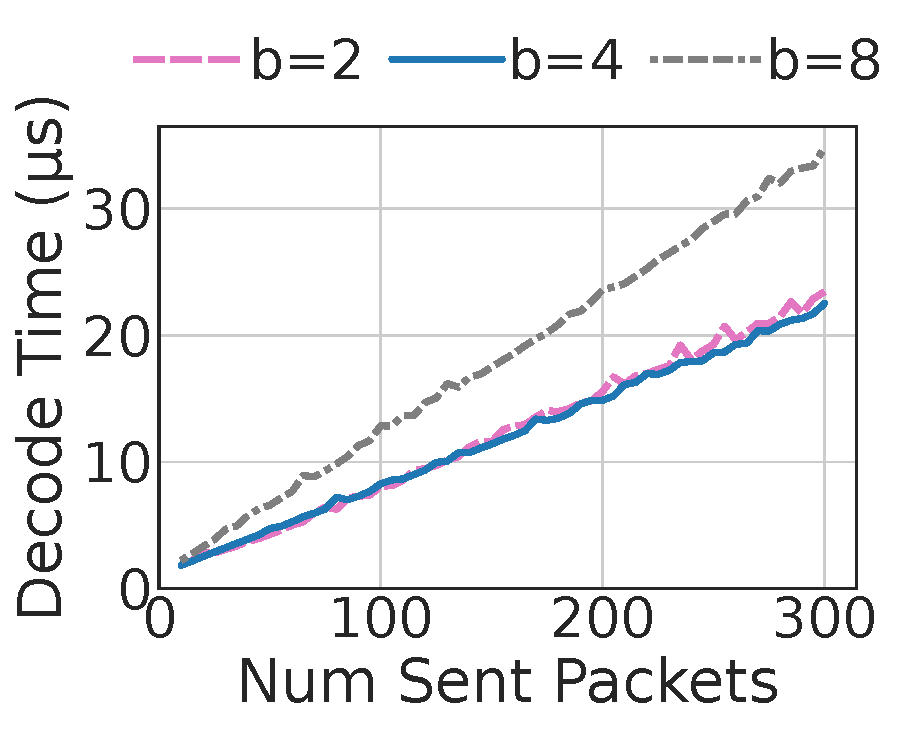
\includegraphics[width=\linewidth,trim={3mm 0 7mm 0},clip]{sidekick-paper/figures/fig2a_quack_num_candidates_vs_decode_time.pdf}
	\caption{\footnotesize Evaluate a degree-$m=t=10$ polynomial at $n$ candidate roots.}
	\label{fig:n-vs-decoding}
\end{subfigure}
\hspace{-0.1em}
\begin{subfigure}{0.32\columnwidth}
	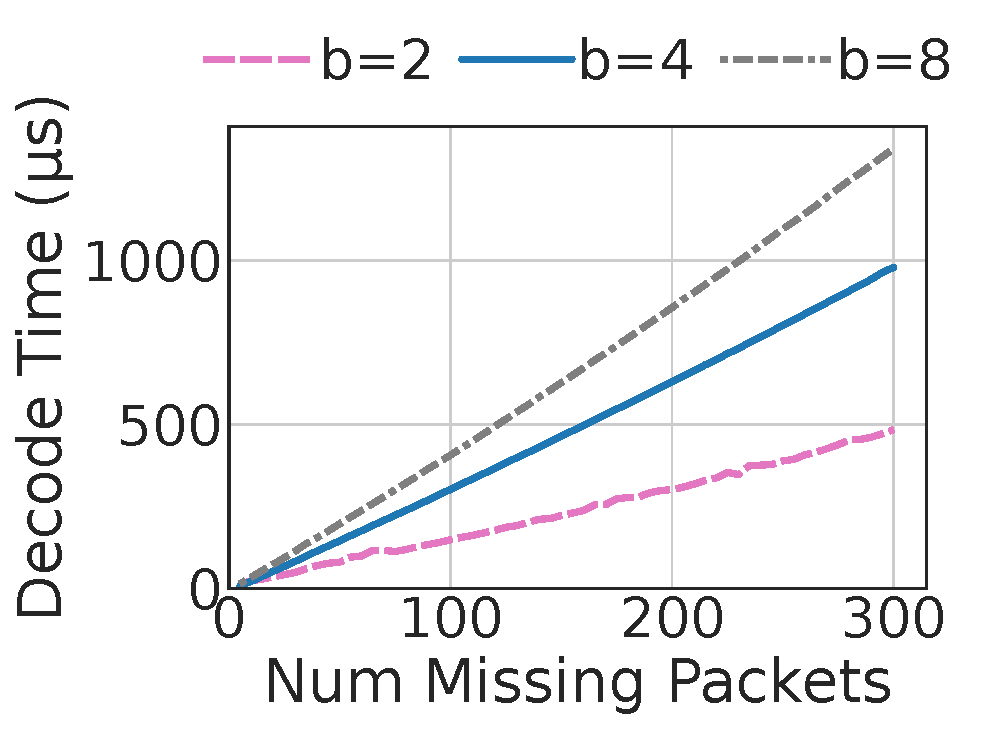
\includegraphics[width=\linewidth,trim={3mm 0 7mm 0},clip]{sidekick-paper/figures/fig2b_quack_num_missing_vs_decode_time.pdf}
	\caption{\footnotesize Plug $n=300$ candidate roots into a degree-$m$ polynomial.}
	\label{fig:m-vs-decoding}
\end{subfigure}
\hspace{-0.1em}
\begin{subfigure}{0.32\columnwidth}
	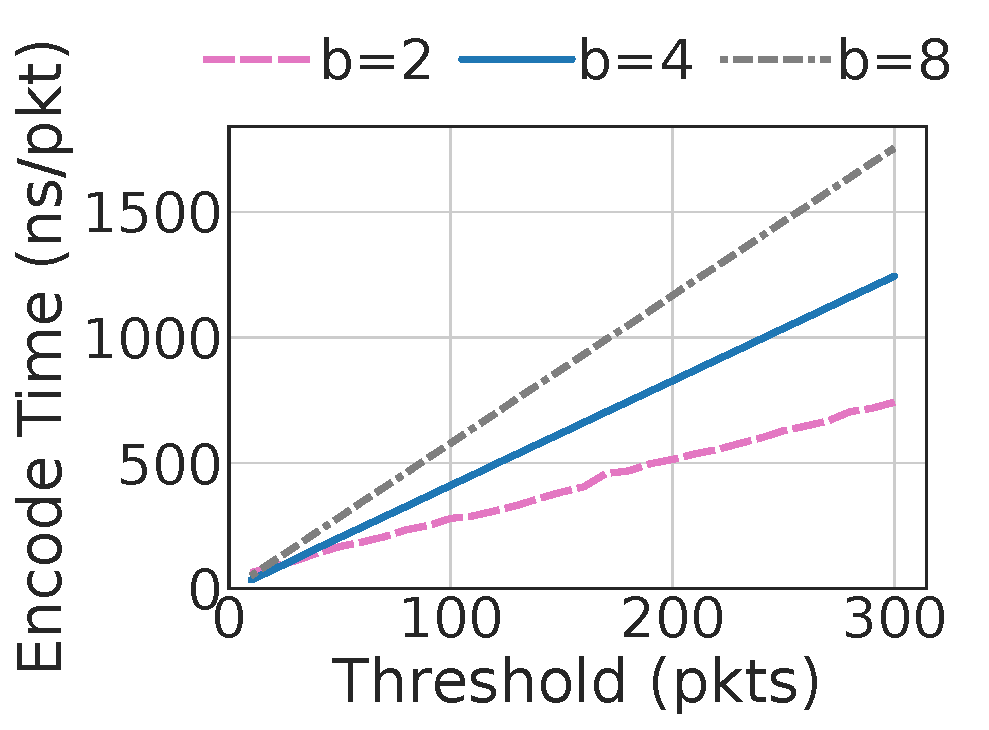
\includegraphics[width=\linewidth,trim={3mm 0 7mm 0},clip]{sidekick-paper/figures/fig2c_quack_threshold_vs_encode_time.pdf}
	\caption{\footnotesize Update $t$ power sum equations.
	Average of $1000$ packets.}
	\label{fig:construction-time}
\end{subfigure}
\vspace{-0.2cm}
\caption{How power sum quACK performance depends on various parameters:
bit width, threshold, number of sent and missing packets.
Average of 100 trials.
\vspace{-0.5cm}
}
\label{fig:quack-plots}
\end{figure}


\subsection{Identifier bit widths}
\label{sec:quack:microbenchmarks:bit-widths}

Different bit widths have different implications for
which instructions the CPU can use. Modular operations are efficient
for 16- and 32-bit integers, fitting within the 64-bit word size (the number of
bits that can be processed in one instruction) of most modern CPUs. For example,
to multiply two 32-bit integers, we cast them to 64-bit integers, multiply,
then take the modulus.

\Cref{fig:quack-plots} shows the best performance we achieved at different bit
widths. For 16-bit identifiers only, we precomputed power tables that fit in
the L3 cache. For 64-bit identifiers, we implemented Montgomery modular
multiplication~\cite{montgomery1985modular} to avoid an expensive hardware
division for 128-bit integers. In the remainder of the paper, we use $b=4$ as
the preferred tradeoff between space and collision probability.

\subsection{Encoding time}
\label{sec:quack:microbenchmarks:encoding}

The encode time per-packet is directly proportional to
the threshold number of missing packets $t$ (\Cref{fig:construction-time}) at
$33/10 \approx 3$ ns/power sum.
Each power sum can be updated in a constant number of operations based on the
previous power sum, so encoding an identifier requires $t$ modular additions
and multiplications for the $t$ power sums.

Encoding in the IBLT is faster in practice when there are at least
$\approx\!30$ symbols (\Cref{fig:quack:encode}).
Each update in the IBLT uses an expensive square root instruction in the
pseudorandom mapping algorithm, adding constant factor overheads that impact
smaller numbers of symbols.

\subsection{Decoding time}
\label{sec:quack:microbenchmarks:decoding}

The decode time must be comparable to the time it takes to process a typical
ACK and modify the logic in the transport protocol. Decoding typically
occurs on end hosts, compared to encoding which occurs in the middle of the path.

Finding the solution to the system of power sum polynomial equations boils down
to applying Newton's identities (a linear algorithm) and finding the roots of a
polynomial equation
in a modular field~\cite{eppstein2011straggler}.
Factoring a polynomial is asymptotically fast in theory, but the implementation
is branch-heavy and complicated~\cite{batut2000user}.
We found that plugging in and evaluating which of $n$ candidate roots
evaluated to zero was faster in practice for $n < 40,000$ roots.
This is the method we use to decode the power sum quACK.

The decode time of this method is directly proportional to $n$ (\Cref{fig:n-vs-decoding})
and the number of missing packets $m$ (\Cref{fig:m-vs-decoding}).
Decoding takes $2820/10/25 \approx 11$ ns/candidate/missing.
Both $n$ and $m$ are typically a few hundred at most.

Decoding in the IBLT is much faster in practice for any number of symbols
(\Cref{fig:quack:decode}). Note that the power sum quACK actually uses a decoding
method that is linear in \textit{all} packets received, not just the \textit
{missing} packets, due to the complexity of symmetric polynomial
factorization.

\subsection{IBLT non-determinism}
\label{sec:quack:microbenchmarks:non-determinism}

\begin{figure}[t]
    \centering
    \begin{subfigure}[b]{0.49\linewidth}
        \centering
        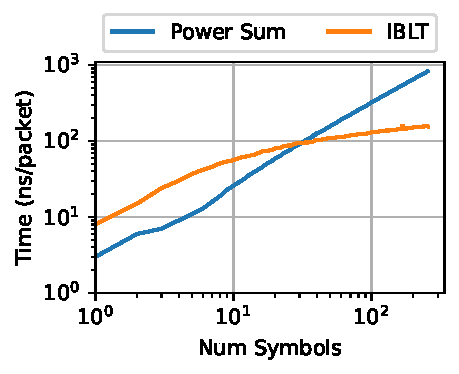
\includegraphics[width=\linewidth]{figures/quack_encode.pdf}
        \caption{Encode time.}
        \label{fig:quack:encode}
    \end{subfigure}
    \begin{subfigure}[b]{0.49\linewidth}
        \centering
        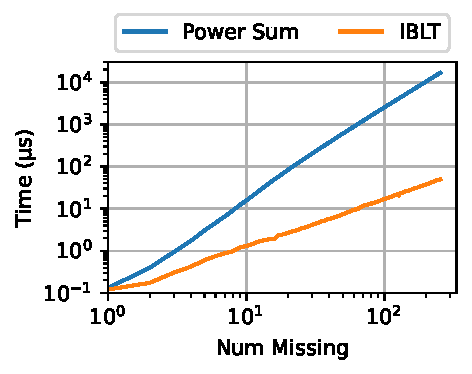
\includegraphics[width=\linewidth]{figures/quack_decode.pdf}
        \caption{Decode time.}
        \label{fig:quack:decode}
    \end{subfigure}
    \caption{IBLT vs. power sum eACK microbenchmarks. The number of trials is
     such that the cumulative time is at least $100$ ms. With rateless eACKs,
     the client can encode much larger numbers of symbols $t$ while the proxy
     decodes fewer symbols in the common case.
     % The logscale axes emphasize the overheads at smaller numbers.
     }
    \label{fig:quack}
\end{figure}
\begin{figure}[t]
    \centering
    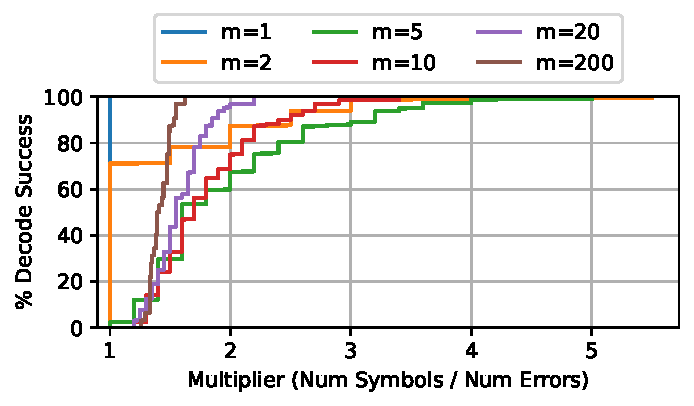
\includegraphics[width=0.9\linewidth]{packrat-paper/figures/quack_multiplier.pdf}
    \caption{The CDF of the minimum number of symbols $t$ needed to successfully
    decode an quACK for various numbers of missing packets $m$, 100000 trials.}
    \label{fig:iblt-quack}
\end{figure}

It is unknown how many symbols are required in the IBLT to decode the same
number of $m$ missing packets using power sums in the previous benchmarks.
There is a constant factor overhead ($1.35\times$ on average~\cite
{yang2024practical}).
\Cref{fig:iblt-quack} shows the CDF of the minimum number of symbols to decode
various $m$ as this constant multiplier increases. $m=1$ trivially requires
one symbol, while the multiplier decreases for higher $m$ to achieve the same
success rates.

The quACK sender does not know how many symbols it needs to encode to later
decode a certain $m$. Using power sums, this is exactly $m$ symbols. In
the quACK, $4 \cdot m$ symbols have at least a $\!98.8\%$ success rate for
all $m$ evaluated in \Cref{fig:iblt-quack}. When $m$ is large, the quACK utilizes more
of the link, but maintaining more symbols at the proxy and client means
the Packrat has a greater worst-case tolerance for errors with the same encoding
overheads. The Packrat proxy can reset the connection if it cannot decode a quACK.

\section{Rateless quACK property}
\label{sec:quack:rateless}

The number of symbols in the quACK is configured for the worst case, but it is
wasteful to consistently send hundreds of bytes over the wire for each quACK.
Unlike set reconciliation in distributed systems, quACKs are transmitted at
millisecond RTT timescales.

In the blockchain setting, the two parties negotiate to determine the number of
missing items, and to send additional symbols if the current number is not
enough to probabilistically decode. This minimizes the number of symbols sent
over the wire, but the in-network retransmission setting does not have the time
to negotiate over multiple RTTs. How else can we apply the rateless property to
quACKs?

In fact, the client can estimate the number of retransmissions it expects from
the proxy and send a smaller quACK, while locally encoding enough symbols for
the worst case. For example, the client can count the number of gaps in an ACK,
or the packets for which it would send a NACK. Both the IBLT and power sums
have the property that a strict prefix of symbols is sufficient to decode a
smaller error.
